\newpage
\maketitle
\begin{center}
\Large \textbf{第1章 强化学习概述} \quad 
\end{center}
\begin{abstract}
在本章中我们将讨论强化学习中的环境、Agent、状态、Action和奖励,并重点讨论MDP相关内容。
\end{abstract}
\section{MDP概述}
一个典型的强化学习系统结构如下所示:
\begin{figure}[H]
	\caption{典型强化学习系统架构图}
	\label{p000001}
	\centering
	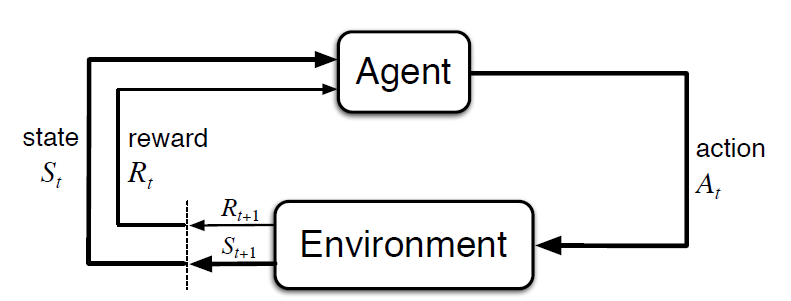
\includegraphics[width=15cm]{images/p000001}
\end{figure}
如图所示:
\begin{enumerate}
    \item 在$t$时刻Agent观察到环境状态$S_{t}$,并得到上一时刻所采取的行动$A_{t-1}$(在图中未画出)所得到的
奖励$r_{t}$;
    \item Agent根据环境状态$S_{t}$,根据某种策略$\pi$,选择行动$A_{t}$;
    \item 环境接收到Agent的行动$A_{t}$后,根据环境的动态特性,转移到新的状态$S_{t+1}$,并产生$R_{t}$的奖励
信号;
\end{enumerate}
\subsection{典型环境}
\subsubsection{Bandit Walk环境}
下面我们来研究一个最简单的强化学习环境,叫Bandit Walk,如下所示:
\begin{figure}[H]
	\caption{Bandit Walk环境图}
	\label{p000002}
	\centering
	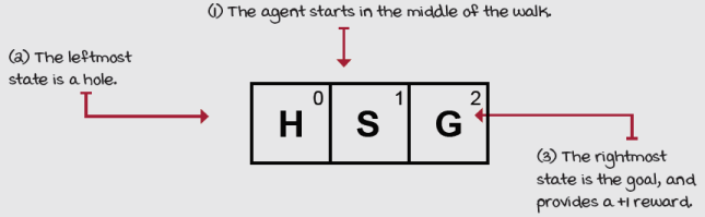
\includegraphics[width=15cm]{images/p000002}
\end{figure}
如图所示,Agent初始时位于中间的S格,状态编号为$S_{0}$,其可以采取向左、向右两个动作,向左则进入状态$H$,其是一个洞,就会掉到洞里,
过程就会结束,此时得到的奖励为0;当Agent采取向右行动时,就会进入G状态,此时会获得奖励+1,由此可见其是一个确定性的环境,就是说当
Agent采取向右行动时,会100\%确定进行G状态。我们可以通过如下的图来表示上述过程:
\begin{figure}[H]
	\caption{Bandit Walk环境MDP图}
	\label{p000003}
	\centering
	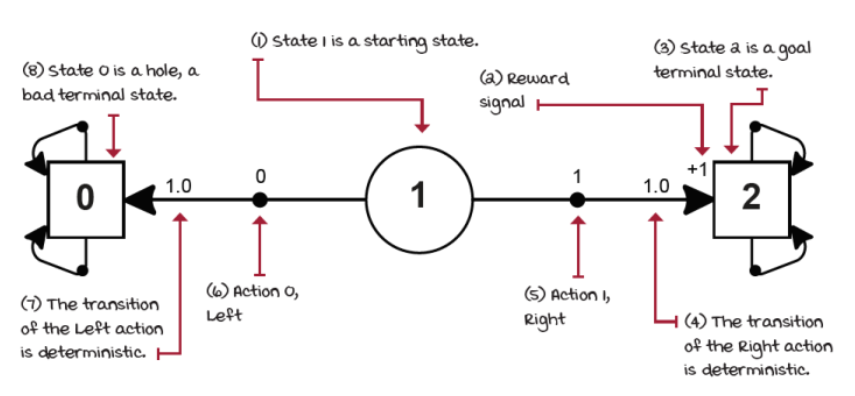
\includegraphics[width=15cm]{images/p000003}
\end{figure}
如图所示:
\begin{itemize}
    \item 在初始状态$S_{0}$时,有两个可选行动,分别表示为向左、向右的直线;
    \item 当采取向右行动时,就会到达小黑点位置,然后由环境决定将转到哪个状态,以及转到这个状态的概率,以本例为例,其就是以100\%
的概率转到G状态$S_{2}$,其中小黑点上面的1代表行动编号,向右简头上面的1.0代表100\%的概率,向右简头处的1代表奖励为+1;
\end{itemize}
我们首先安装所需要的库:
\lstset{language=PYTHON, caption={安装gmy库}, label={pip-install-gym}}
\begin{lstlisting}
pip install gym -i https://pypi.tuna.tsinghua.edu.cn/simple 
\end{lstlisting}
下面我们用Python对象来表示这一过程:
\lstset{language=PYTHON, caption={Bandit Walk python程序}, label={bandit-walk-python-env}}
\begin{lstlisting}
P = {
    0: {
        0: [(1.0, 0, 0.0, True)],
        1: [(1.0, 0, 0.0, True)]
    },
    1: {
        0: [(1.0, 0, 0.0, True)],
        1: [(1.0, 2, 1.0, True)]
    },
    2: {
        0: [(1.0, 2, 0.0, True)],
        1: [(1.0, 2, 0.0, True)]
    }
}
print(P)
\end{lstlisting}
代码解读如下所示:
\begin{itemize}
    \item P为一个字典对象,其键值0、1、2代表三个状态;
    \item P的键值0:其同样是一个字典对象,键值代表可以采取的行动,0代表向右,1代表向右;
    \item P的键值0下键值0:即在状态0下面采取行动0,其值为一个数组,代表由环境决定要转到哪个状态,转到每个状态为一个Turple,含
义为:(概率, 目的状态,获得奖励,新状态是否为终止状态),注意:我们规定在终止状态采取任何行动都会回到自身;
\end{itemize}
上面我们仅举了一个例子,其他状态读者可以自己解析出来。
\subsubsection{Bandit Slippery Walk环境}
在上面的环境中,我们向左移动,环境会确定地向左移动。但是在本节中,当我们向左移动时,环境在80\%的情况下会向左移动,20\%的情况会
向右移动。如下图所示:
\begin{figure}[H]
	\caption{Bandit Slippery Walk环境图}
	\label{p000004}
	\centering
	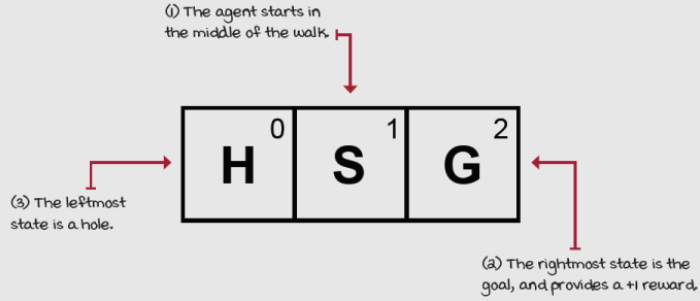
\includegraphics[width=15cm]{images/p000004}
\end{figure}
除了环境的随机性之外,环境与上一节相同。其MDP图如下所示:
\begin{figure}[H]
	\caption{Bandit Slippery Walk环境MDP图}
	\label{p000005}
	\centering
	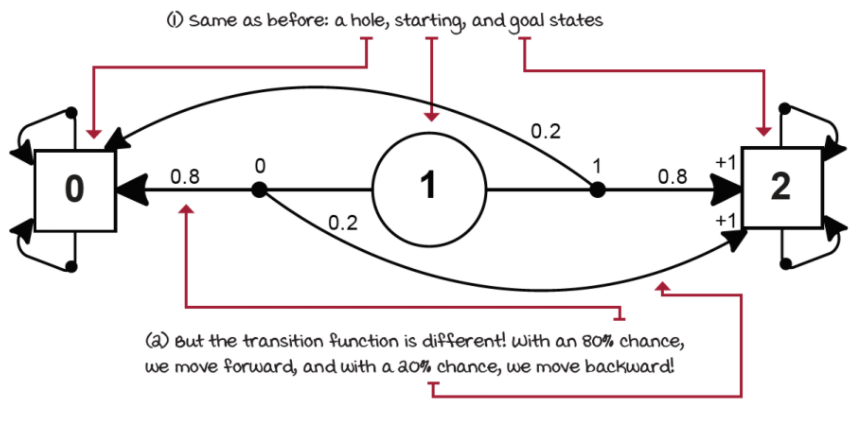
\includegraphics[width=15cm]{images/p000005}
\end{figure}
如上图所示,在开始时Agent位于状态S,其可以采取的行动为向左编号为0或向右编号为1,我们以向右为例,当Agent采取向右行动时,其达到状态S右侧的小黑点,上面的1代表是编号为1的行动,
此时环境将以80\%的概率转变为状态G,得到+1的奖励,如图中的右箭头所示,同时环境还可能将以20\%的概率变为状态H,其所获得的奖励为0,如图中向左的曲线箭头所示。读者可以按照上面
的描述,自己补充出其他状态变化情况。由前面的讨论可以看出,在这个例子中,当Agent采取向右行动Action时,环境仅以80\%的概率完成该Action,同时还可能以20\%的概率向相反的方向
变化,既环境具有一定的随机性。
我们可以通过如下的Python代码来表示这一过程:
\lstset{language=PYTHON, caption={Bandit Slippery Walk python程序}, label={bandit-slippery-walk-python-env}}
\begin{lstlisting}
    def bandit_slippery_walk(self):
        P = {
            0: {
                0: [(1.0, 0, 0.0, True)],
                1: [(1.0, 0, 0.0, True)]
            },
            1: {
                0: [(0.8, 0, 0.0, True), (0.2, 2, 1.0, True)],
                1: [(0.8, 2, 1.0, True), (0.2, 0, 0.0, True)]
            },
            2: {
                0: [(1.0, 2, 0.0, True)],
                1: [(1.0, 2, 0.0, True)]
            }
        }
        print(P)
\end{lstlisting}
如上所示,在状态S时,如果采取编号为0的向左行动,则有80\%的概率会进入到状态H,奖励为0.0,并且是终止状态,当采用编号为1的向右行动时,将进入状态G,获得奖励为1.0,并且为终止状态,
采用这种方式我们就表示了环境的随机性。
\subsection{典型交互}
Agent与环境的交互分为分段的或连续的,由一系列时间步聚组成,在时间$t$时刻:
\begin{itemize}
    \item Agent得到环境给的奖励信号$R_{t}$,其由Agent在上一时刻$S_{t-1}$采取行动$A_{t-1}$时所获得的,并且Agent观察到环境状态$S_{t}$;
    \item Agent根据所观察到的环境状态$S_{t}$,选择采取行动$A_{t}$;
    \item 环境接收到行动$A_{t}$后,会转移到新的状态$S_{t+1}$,并且会给Agent奖励$R_{t+1}$;
    \item 依次循环......
\end{itemize}
上述过程可以表示为:
\begin{equation}
\begin{aligned}
(R_{0}, S_{0}, A_{0}), (R_{1}, S_{1}, A_{1}), (R_{2}, S_{2}, A_{2}), ..., (R_{t}, S_{t}, A_{t}), ..., (R_{T}, S_{T}, A_{T})
\end{aligned}
\label{mdp-episode-trajectory}
\end{equation}
\subsection{MDP定义}
我们以Frozen Lake为例来定义MDP过程。该环境如下所示:
\begin{figure}[H]
	\caption{Frozen Lake环境图}
	\label{p000006}
	\centering
	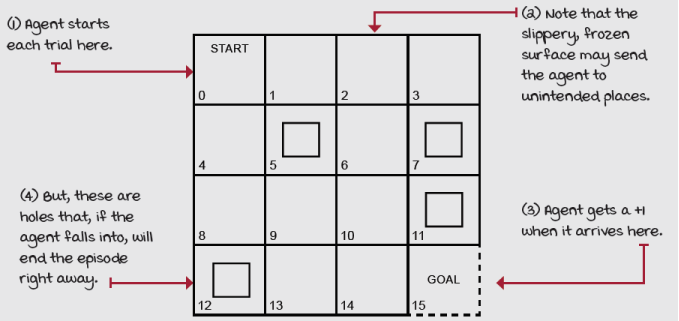
\includegraphics[width=15cm]{images/p000006}
\end{figure}
如图所示:
\begin{itemize}
    \item Agent从状态Start开始;
    \item 在每个状态,Agent可以采取向左、向上、向下、向右行动,当在边缘状态时,走出环境的行动会100\%使Agent留在原状态;
    \item 由于是冻冰的湖面,例如当Agent选择向下行动时,其有33.3\%的概率向下运动,还有66.7\%的概率会向垂直的方向运动,既以33.3\%的概率向左运动,33.3\%的概率向右运动;
    \item 当Agent到达有洞的状态时,过程立即结束;
    \item 当Agent到达最终节点时,可以获得+1的奖励;
\end{itemize}
\subsubsection{环境状态建模}
时刻$t$环境状态的状态表示为$S_{t}$,环境所有可能的状态用集合$\mathcal{S}$表示,通常我们用$n$维向量来表示一个状态:
\begin{equation}
\begin{aligned}
S_{t}=\boldsymbol{s} = \begin{bmatrix}
    s_{1} \\
    s_{2} \\
    ... \\
    s_{n}
\end{bmatrix} \in R^{n}
\end{aligned}
\label{state-vector-representation}
\end{equation}
对于我们当前研究的这个问题,环境状态只需要表示Agent处于哪个状态即可,我们采用0$\sim$15来对状态进行编号,因此状态可以用0$\sim$15来表示:
\begin{equation}
\begin{aligned}
S_{t}=\boldsymbol{s} = \begin{bmatrix}
    i
\end{bmatrix} \in R^{1}, i \in \{0, 1, 2, 3, ..., 15\}
\end{aligned}
\label{frozen-lake-state-demo}
\end{equation}
我们规定环境只与当前状态有关,而与过去的历史无关,这就是马可夫特性,即我们研究的过程是无记忆的。乍一看,这是一个非常严重的限制条件,但是在实际应用中,我们通常可以通过设计合适的状态,使
所研究的问题变为无记忆的。用数学语言可以表示为:
\begin{equation}
\begin{aligned}
P(S_{t+1} | S_{t}, A_{t}) = P(S_{t+1} | S_{t}, A_{t}, S_{t-1}, A_{t-1}, ...)
\end{aligned}
\label{markov-property-def}
\end{equation}
以Frozen Lake为例,其每个状态和在状态上可以采取的行动如下所示:
\begin{figure}[H]
	\caption{Frozen Lake状态和行动图}
	\label{p000007}
	\centering
	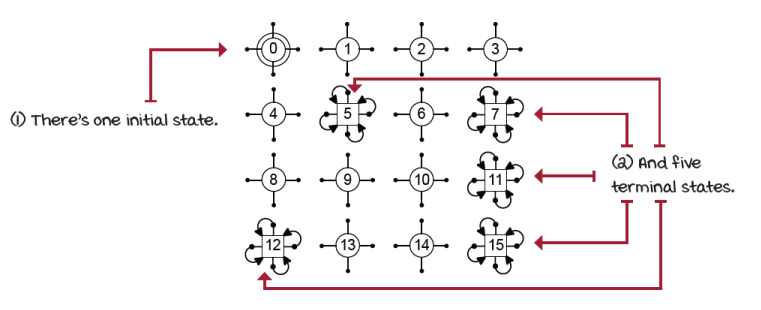
\includegraphics[width=15cm]{images/p000007}
\end{figure}
当Ageng采取行动后,环境会根据自身的动态特性,转移到下一个状态,我们称之为转移函数,如下图所示:
\begin{figure}[H]
	\caption{Frozen Lake状态转移图}
	\label{p000008}
	\centering
	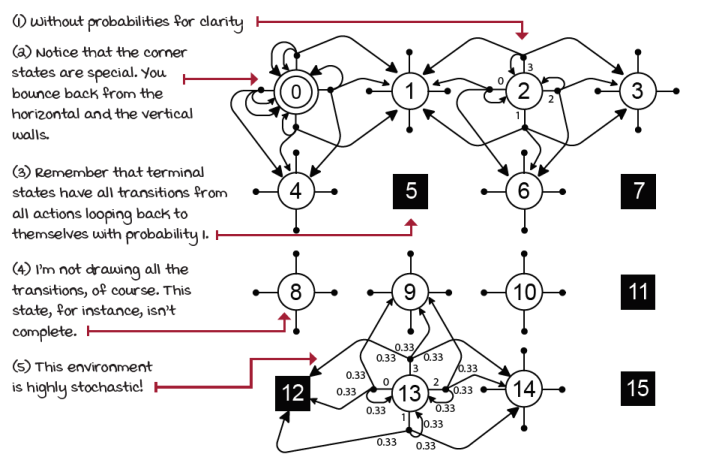
\includegraphics[width=15cm]{images/p000008}
\end{figure}
在状态13时,共有向左、向下、向右、向上编号分别为0、1、2、3的四种行动,当Agent采取行动0向左时,将到达左侧的小黑点,
\begin{itemize}
    \item 行动0(向左):到达左侧小黑点,由于冻冰原因,其有如下三种可能性:
    \begin{itemize}
        \item 33.3\%:向左,进入状态12,获取奖励0.0,并且为终止状态,用(0.333, 12, 0.0, True)表示;
        \item 33.3\%:向下,由于是边缘节点,其仍然在状态13,获取奖励0.0,不为终止状态,用(0.333, 13, 0.0, False)表示;
        \item 33.3\%:向上,进入状态9,获取奖励为0.0,不是终止状态,用(0.33, 9, 0.0, False)表示;
    \end{itemize}
    \item 行动1(向下):到达下面小黑点,有如下三种可能性:
    \begin{itemize}
        \item 33.3\%(向下):由于是边缘节点,其仍然在状态13,获得奖励为0.0,不是终止状态,用(0.333, 13, 0.0, False)表示;
        \item 33.3\%(向左):进入状态12,获得奖励0.0,并且为终止状态,用(0.333, 12, 0.0, True)表示;
        \item 33.3\%(向右):进入状态14,获得奖励0.0,不是终止状态,用(0.333, 14, 0.0, False)表示;
    \end{itemize}
\end{itemize}

